\chapter{Synthèse des activités de recherches} % Main chapter title

\label{synthese} % For referencing the chapter elsewhere, use \ref{Chapter1}

\section{Préabule et déroulement de carrière}
J’ai un parcours scientifique atypique qui s’est construit sur un cursus universitaire alternant formations diplômantes et expériences professionnelles. Mes premiers contacts avec le monde de la recherche scientifique date de 1998. Après une maîtrise de biochimie, j’ai eu l’opportunité de travailler sur des protocoles expérimentaux en biologie moléculaire au sein d’équipes de recherche de l’INRA. En 1999, j’ai poursuivi ces expériences professionnelles au CIRAD pour développer et analyser une banque de marqueurs microsatellites chez le cacao. J’ai pu alors constater l’importance de l’informatique pour la gestion et le traitement des données à l’échelle de la biomolécule. Un tel constat m’a conduit à compléter ma formation de biologiste avec une année de DESS en informatique. J’ai pu alors aborder les problématiques associées à l’organisation et au traitement des données moléculaires sous un angle nouveau lors du stage de fin de cursus du DESS en 2000, qui s’est déroulé dans la même unité de recherche. \\

Mon parcours scientifiaue a démarré en 2001, en tant qu’ingénieur d’étude en bioinformatique dans le groupe d’E. Guiderdoni au CIRAD (UMR AGAP) dans le contexte du projet ANR Génoplante « Analyse fonctionnelle du génome du riz : création d'une collection de 15.000 lignées de mutants d'insertion de riz ».  L'objectif de ce projet était de créer et caractériser une collection de mutants T-DNA chez la variété O. sativa ssp nipponbarre. Le projet était très ambitieux sur le plan informatique et comprenait en effet tous les aspects de traitement de séquences génomiques mais aussi l’informatisation des processus d’analyse phénotypique (qui relèvent de ce que l’on appelle aujourd’hui le phénome). Un défi du projet portait sur la mise en place d’un système intégré, pouvant répondre aux attentes de différentes  équipes de recherche localisées sur différents sites géographiques. Très rapidement mes activités ont concerné des problèmes qui au-delà de la haute technicité impliquaient des réflexions méthodologiques liées à la gestion de données et de connaissances hétérogènes. C’est dans ce contexte que j’ai effectué ma thèse. J’ai bénéficié de l’encadrement  de Thérèse Libourel ( Pr. LIRMM, directeur ), d’Isabelle Mougneot (Mdc LIRMM - Univ. Montpellier) et Manuel Ruiz (Chercheur Cirad). D’un point de vue méthodologique, j’ai défini une structure de médiation (paradigme médiateur/adaptateur) reposant sur un schéma global construit sur l'ensemble des vues sur les schémas sources permettant une consultation unifiée de différentes sources de données hétérogènes dans le contexte de la génomique fonctionnelle. Le médiateur mis en place s’appuyait sur l’approche GAV (Global As View) avec un ensemble de vues sur les schémas des sources de données qui tient lieu de schéma global. J’ai obtenu un poste d’ingénieur d’études CNRS dans l’équipe “Intégration des Données” (ID) dirigée par M. Ruiz au CIRAD (UMR AGAP) quelques temps avant de soutenir ma thèse. \\

J’ai poursuivi dans cette voie autour des méthodes d’intégration de données dans le domaine agronomique et je me suis par ailleurs impliqué dans l’animation de la plateforme bioinformatique South Green.  \\
Je me suis d’abords orienté sur le développement de méthodes automatisant la création d’adaptateurs sémantiques et la formulation de requêtes pour des bases de données biologiques en co-encadrant la thèse de Julien Wollbrett (voir section \ref{SWS}).\\

Par la suite, j’ai quitté le CNRS en 2010, pour effectuer une mobilité au sein de l’IRD dans l’équipe Génome et Développement du Riz (UMR DIADE) dont les enjeux en matière de partage et d’intégration de données génomiques étaient particulièrement motivants. Je me suis également fortement impliqué dans la structuration d’une plateforme bioinformatique naissante transversale sur plusieurs unités IRD. \\
Afin de répondre aux besoins de gestion des masses de données produites par le séquencage et le phénotypage de nouvelles variétés de riz, j’ai développé des méthodes d’intégration et de stockage basées sur des architectures distribuées détaillées en section \ref{GIGWA}. \\
Depuis 2012, je suis impliqué dans le projet « Institut de Biologie Computationnelle » (IBC). IBC est un projet ANR « investissement d’avenir » en bioinformatique dont l’objectif est de développer de nouvelles méthodes et logiciels pour le traitement des grandes masses de données biologiques avec des applications dans les domaines de la santé, l’agronomie et l’environnement. 
Jusqu'en 2016, j'ai été co-responsable de l’axe « intégration des données et connaissances biologiques » qui reprend les problématiques d’intégration de données pour la biologie des plantes. Je me suis fortement impliqué dans cette tâche car les problématiques sont très importantes pour l’unité DIADE. Pour mener à bien cette coordination, j’ai partagé mon temps entre les locaux d’IBC situé au LIRMM et l’équipe RICE. J’ai pu ainsi créer une synergie entre experts de différents domaines de l’informatique et de la biologie afin d’avancer sur des points tels que la gestion des données phénomiques et la gestion des données NGS (Next Generation Sequencing). Mes activités de recherches menées dans le cadre du projet IBC sont décrites en section \ref{IBC}. \\
## Depuis le mois de septembre 2016, je travaille mandaté par l'IRD en expatriation au Vietnamß pour développer in situ des approches bioinformatiques avec les partenaires Vietnamiens du LMI RICE\footnote{\url{https://sites.google.com/site/lmiricevn}}, afin de permettre une meilleure exploitation de leurs données. Récemment, j’ai pris la responsabilité du laboratoire informatique IRD-USTH (Université des Sciences et Techniques d’Hanoi). Le laboratoire compte neuf jeunes enseignants chercheurs en informatique avec qui je collabore sur certains aspects méthodologiques. Par ailleurs, je consacre une partie de mon temps à l’enseignement en Masters (Informatique et Biologie) ainsi qu’à l’encadrement d’étudiants. Je développe également des collaborations avec l’ International Rice Research Institute (IRRI) qui est un des centres du Consultative Group on International Agricultural Research (CGIAR) sur le Riz basé aux Philippines.


\section{Activités de recherche en cours}

Les progrès de la génomique et des outils de phénotypage à haut débit offrent une occasion unique de découvrir de nouveaux gènes. Les ressources génétiques peuvent maintenant être séquencées à faible coût pour étudier de manière fine leur diversité génétique. Les systèmes d'information actuels permettent de plus en plus l'intégration de données hétérogènes, cependant de nombreux challenges existent encore lorsqu'ils s'agit d'exploiter le croisement de ces données d'autant plus que ces données sont massives et multi-échelles. De nombreux challenges résident dans le traitement de l'information sous-jacente afin de découvrir rapidement des relations gène-phénotype et leur dépendance à l’environnement qui détermine le rendement des cultures dans des environnements divers.

\subsection*{Mise en place d’approches pour l’interopérabilité des bases de données biologiques}

Dans le contexte du projet Genoplante, la caractérisation de la collection de mutant comprenait le séquençage des gènes discutés par le TDNA (et les autres éléments mobiles) ainsi que la caractérisation phénotypique des lignées de mutants sur plusieurs sites géographiques. J'ai eu la charge du volet bio-informatique. J'ai ainsi développé un workflow de détection et d'annotation des séquences nucleotidiques (2004-02). J'ai également été impliqué, dans le développement de l'application OrygenesDB \footnote{\url{http://orygenesdb.cirad.fr}}, une application web permettant de stocker des données relatives aux séquences générées lors du projet et également les séquences issues du séquençage du génome du riz (2006-01). Le principal objectif de mon travail a été la conception du système d'information dédié à la gestion des données phénotypiques et leur enrichissement par des liens avec les autres ressources (génomique, transcriptomique, protéomique) décrivant la collection. Pour ce faire, j’ai développé OryzaTagLine \footnote{\url{http://oryzatagline.cirad.fr}}, un système d’information permettant d’intégrer et centraliser ces différentes ressources afin de fournir un portail web unique aux scientifiques (2008-01)\\

Au cours de ce projet, je me suis engagé sur une thèse afin de lever de nombreux verrous liés à l’intégration de données dans le domaine agronomique. Les thématiques abordées concernaient (i) la formalisation de standards d’échange de données, de métadonnées et d’ontologies pour décrire et annoter les données, (ii) le développement d’infrastructures permettant la communication d’applications sur des réseaux distribués. L’objectif de mon travail était de permettre aux scientifiques d'accéder de manière transparente aux informations issues de plusieurs sources de données (génomique, phénotypique, etc.).  Pour cela, j’ai abordé le sujet en développant deux approches : une architecture de médiation et une architecture orienté services (SOA).  La première proposait l’intégration de sources à travers l'adaptation d'un système de médiation de données : Le Select~\cite{manolescu2002}. Successeur de DISCO~\cite{Tomasic1998}, Le Select utilisait un modèle pivot relationnel afin d’intégrer de manière transparente les sources de données hétérogènes et distribuées. La deuxième, proposait l’intégration des sources à travers l’enchainement de services web grâce à un environnement web personnalisé (2008-02). Ce système utilisait le Framework BioMoby~\cite{Wilkinson2002a,Wilkinson2005a}  et son annuaire de services bioinformatiques. \\

Mes contributions ont permis de généraliser l’utilisation des standards d’échanges de données (au sein du CIRAD et de ses partenaires) ainsi que d’appliquer différentes approches d’intégration de données en agronomie. Elles ont également permis d’accroitre les fonctionnalités des applications OryzaTagLine et OrygenesDB et leur interopérabilité avec d’autres systèmes existants.

\subsubsection*{Sélection de références}

\begin{itemize}

\item (2004-02) Sallaud C., Gay C., Larmande P., Bès M., Piffanelli P., Piégu B., Droc G., Regad F., Bourgeois E., Meynard D., Périn C., Sabau X., Ghesquière A., Delseny M., Glaszmann J.C., Guiderdoni, E. (2004) High throughput T-DNA insertion mutagenesis in rice : A first step towards in silico reverse genetics. Plant J. 2004 Aug; 39(3):450-64. Impact Factor: 5.468      
\item (2006-01) Droc G, Ruiz M, Larmande P, Pereira A, Piffanelli P, Morel JB, Dievart A, Courtois B, Guiderdoni E, Périn C. OryGenesDB: a database for rice reverse genetics. Nucleic Acids Res. 2006 Jan 1; 34(Database issue):D736-40. Impact factor: 9.202
\item (2008-01) Larmande P, Gay C, Lorieux M, Périn C, Bouniol M, Droc G, Sallaud C, Perez P, Barnola I, Biderre-Petit C, Martin J, Morel JB, Johnson AA, Bourgis F, Ghesquière, A, Ruiz M, Courtois B, Guiderdoni E. Oryza Tag Line, a phenotypic mutant database for the Genoplante rice insertion line library. Nucleic Acids Res. 2008 Jan; 36(Database issue):D1022-7. Impact factor: 9.202 
\item (2008-02) Droc G, Périn C, Fromentin S, Larmande P. OryGenesDB 2008 update: database interoperability for functional genomics of rice. Nucleic Acids Res. 2009 Jan; 37 (Database issue):D992-5. Impact factor: 9.202

\end{itemize}

\subsection*{Génération automatique de services web pour les bases de données relationnelles biologiques}
\label{SWS}

Ayant rejoint l’équipe intégration des données de M. Ruiz, j’ai été impliqué dans le projet international Generation Challenge Programme (GCP), l’un des cinq Challenge Programme établis par le Consultative Group on International Agricultural of Research (CGIAR).  \\ %## Ici tu donnes le détail .... ##

Une plateforme d’intégration de données, nommée GCP Pantheon, avait été développée afin de permettre à des clients logiciels d’interroger de manière transparente tout type de données générées dans le cadre du programme GCP. Cette plateforme combinait une approche de médiation LAV (Local As View) et une approche sémantique, permettant aux partenaires de gérer leurs données localement puis de les rendre accessibles facilement en accord avec un modèle conçu spécifiquement pour le projet, GCP Domain Model~\cite{Bruskiewich2006,Bruskiewich2008}. Le modèle GCP a également été utilisé pour implémenter le Framework BioMoby qui s’était rapidement imposé comme protocole standard d’échanges de données et de services dans le domaine bioinformatique.\\

La principale limitation de la plateforme GCP Pantheon était due au « mapping » manuel des schémas des sources locales sur le schéma global du GCP Domain Model. Afin de lever cette limitation, j’ai co-encadré une thèse (thèse de Julien Wollbrett) sur les méthodes de création automatique d’adaptateurs, facilitant ainsi l’intégration sémantique des bases de données relationnelles biologiques sur la GCP. A cet effet, la thèse exploitait l’utilisation de différentes ontologies de domaines (génomique, phénotypiques, etc.) permettant l’établissement à la fois des règles de correspondance et d’interprétation, nécessaires à l’intégration automatisée. 

Le point commun de l’intégration de données et des technologies du Web Sémantique est de dépasser l’hétérogénéité sémantique de sources de données interconnectées. Le Web Sémantique facilite la représentation de la sémantique des données et peut ainsi être utilisé pour faciliter l’interopérabilité ou l’intégration de données~\cite{antezana2009,Jonquet2010}. %## Peut être bien expliquer que parmi les standards du web semantique on trouve RDF qui est très souvent utilisé pour formaliser les données et ensuite dire que D2RQ est une plateforme qui permet d'accéder aux SGBD relationnels via une vision RDF. ##

L'intégration de base de données relationnelles (BDR) en utilisant les standards du Web Sémantique est confrontée à une problématique de mise en correspondance (mapping) entre des schémas de BDR et une ou plusieurs ontologies. Dans notre approche nous avons décidé de détourner l'utilisation d'un outil de mapping entre schémas de BDR et ontologies nommé D2RQ~\cite{Bizer2003,Bizer2004} pour, en plus d'homogénéiser des schémas hétérogènes, automatiser la création de requêtes sur des BDR distribuées. Pour cela nous avons enrichi sémantiquement et de manière automatique la vue RDF du schéma de BDR créée par D2RQ. Nous avons ensuite travaillé sur la formulation de requêtes se basant sur les vues RDF ainsi générées en développant un algorithme de recherche de plus court chemin dans les graphes RDF~\cite{wollbrett2013clever} capable de prendre en compte les particularités des schémas relationnels. Nous avons ainsi, développé BioSemantic, une approche flexible, générique et automatisée en nous appuyant sur des standards du Web Sémantique et des Services Web (2013-01). 

\subsubsection*{Sélection de références}

\begin{itemize}

\item (2013-01) Wollbrett J, Larmande P, De Lamotte F, Ruiz M. Clever creation of rich SPARQL queries from annotated relational schema: application to Semantic Web Service creation. BMC Bioinformatics. 2013. Impact Factor: 2.435
\end{itemize}

\subsection*{Passage à l’échelle dans l’analyse des variations génomiques}
\label{GIGWA}

Les enjeux du stockage et traitement des données génomiques sont au cœur des problématiques de l’unité DIADE IRD. L’équipe RICE coordonne le projet IRIGIN (International RIce Genomic Initiative) dont l’objectif est de réaliser le re-séquençage de centaines de variétés de riz et le génotypage par séquençage de milliers de lignées de riz, avec l’équivalent de 18 000 génomes de riz en termes de volume de données (90 TeraBytes). Aujourd'hui bien que les biologistes ont souvent encore l'habitude de manipuler leurs données à l'aide de logiciels de type tableur, les données devenant massives et complexes leurs en limite l'utilisation. Les alternatives sont souvent l’utilisation des logiciels exécutables lignes de commande dans un environnement Unix.
Depuis 2013, je coordonne le développement d’un logiciel nommée Gigwa qui facilite cette tâche. Gigwa est une application qui utilise la technologie de base de données NoSQL (MongoDB) afin de gérer le passage à l’échelle pour le stockage et l’analyse des données de variations génomiques (typiquement issus de fichiers VCF, standard de représentation des variants génomiques), et d’offrir une interface WEB permettant d’y appliquer des filtres. Ce système permet alors de naviguer dans les résultats et de ré-exporter ces sous-jeux de données sous divers formats standardisés et de visualiser les variations dans leur contexte génomique. La contribution novatrice dans ce projet réside dans le modèle de stockage de données, que nous avons défini et optimisé pour ce type de données. De plus, le modèle tire avantage de la flexibilité d’extension du SGBD et permet d’utiliser l’application sur un ordinateur de bureau comme sur un cluster de calcul en distribuant les données sur plusieurs nœuds. Bien entendu, les performances tiennent compte du volume de données stockées et des ressources allouées, mais nous obtenons des résultats encourageant par rapport aux autres applications leader dans ce domaine. Un article effectuant le comparatif vient d’être récemment publié (2016-01).


Actuellement, nous développons une API de services REST pour Gigwa comme alternative à son interface web. Cette API qui respecte et étend les recommandations du GA4GH Data Working Group\footnote{\url{http://ga4gh.org}} permettra d’accroitre l’interopérabilité de l’application avec d’autres systèmes utilisés dans la communauté bioinformatique tels que Galaxy~\cite{Giardine2005,Goecks2010}, FlapJack~\cite{Milne2010}, SniPlay~\cite{Dereeper2015} ou Toggle~\cite{Monat2015}.


En perspective d’extraire de la connaissance dans cette masse d’information génomique, nous avons commencé à explorer les possibilités que peuvent offrir les approches de « mapping » entre le web sémantique et les bases de données NoSQL orientées documents (e.g., MongoDB). Dans le cadre du projet spirale IRD BIOeSAI, un système d’information a été développé pour stocker les données expérimentales (i.e. génomique, phénotypique, etc.) en utilisant MongoDB (2015-01). La phase exploratoire du projet a consisté dans l’évaluation de plusieurs approches pour mapper le schéma du système à un modèle RDF annoté avec des ontologies biologiques~\cite{Luyen:2016} (2016-02).



\subsubsection*{Sélection de références}

\begin{itemize}
\item (2016-01) Sempéré G, Philippe F, Dereeper A, Ruiz M, Sarah G, Larmande P. Gigwa—Genotype investigator for genome- wide analyses. Gigascience. 2016. 5:25. Impact Factor : 7.463
\item (2016-02) Le Ngoc L, Tireau A, Venkatesan A, Neveu P, Larmande P. Development of a knowledge system for Big Data: Case study to phenotyping data. Int. Conf. Web Intell. Min. Semant. Proceedings ACM WIMS ’16. 2016. Nimes (France)
\item (2015-01) Le Ngoc L., Jouannic S. and Larmande P. Développement d'un outil générique d'indexation pour optimiser l'exploitation de données biologiques. Poster aux Journées ouvertes pour la Biologie, l’informatique et les Mathematiques JOBIM 2015. Clermont-Ferrant (France)
\end{itemize}


\subsection*{Intégration sémantique des données agronomiques}
\label{IBC}

Depuis 2013, je suis impliqué dans le projet « Institut de Biologie Computationnelle » (IBC). Je suis coordinateur de l’axe « intégration des données et connaissances biologiques » qui reprend les problématiques d’intégration de données pour la biologie des plantes.

Nous avons dans un premier temps, contribué au développement de méthodes automatiques d’intégration de bases de données biologiques en associant les logiciels WebSmatch~\cite{Coletta2012}, développé par l’équipe INRIA Zénith, Bioportal~\cite{Noy2009,Melzi} et Biosemantic~\cite{wollbrett2013clever} en réalisant un prototype~\cite{castanier2014semantic}. Ce travail a permis d’identifier un besoin dans l’annotation sémantique des données et la gestion des ontologies pour le domaine des plantes. \\

Avec Clément Jonquet (MdC Lirmm), nous avons réalisé un premier prototype d’entrepôt d’ontologie nommé AgroPortal. Le projet Agroportal vise à développer un portail d'ontologies de référence pour le domaine de l'agronomie. Une première version de la plateforme est d’ores et déjà déployée et maintenue sur un serveur du LIRMM \footnote{\url{http://agroportal.lirmm.fr}}. \\

La plateforme AgroPortal~\cite{Jonquet2016} reprend la technologie du NCBO BioPortal (portail pour la santé et les ontologies biomédicales, \footnote{\url{http://bioportal.bioontology.org}}. Cette technologie est open-source et indépendante du domaine thématique concerné. Le portail propose des services de recherche d'ontologie et de visualisation, avec la possibilité de déposer des commentaires et des notes. Il offre également un service d'annotation sémantique de données avec les ontologies. L'objectif principal de ce projet est de permettre une utilisation simple des ontologies liées au domaine de l'agronomie, en proposant aux chercheurs de prendre en charge les questions d'ingénierie des connaissances complexes pour annoter les données de recherche. De nombreuses contributions scientifiques ont été réalisées pour améliorer les fonctionnalités du portail. Des nouvelles méthodes de scores~\cite{Melzi} ont été développées pour classer les mappings avec des termes ontologiques. Un nouvel algorithme de recommandation a été implémenté dans le \textit{Recommender}~\cite{RomeroJOGPM16} et un nouveau modèle de métadonnées a été développé et implémenté dans la plateforme~\cite{toulet:lirmm-01397388}.\\

Les données ainsi annotées semantiquement nécessitaient une infrastructure permettant de les gérer efficacement. Or, il n’existait pas d’application de ce type dans le domaine agronomique. Avec l’aide d’un post-doctorant recruté dans le projet IBC en 2014, nous avons élaboré des modèles de données et développé un premier prototype de système d’intégration sémantique de ressources biologiques (AgroLD\footnote{\url{http://www.agrold.org}}). AgroLD est une base de connaissance utilisant les technologies du web sémantique comme structure pour intégrer les données. AgroLD est conçue pour intégrer des informations disponibles sur diverses espèces végétales. Le cadre conceptuel de la connaissance est basé sur des ontologies bien établies dans le domaine. En outre, compte tenu de la portée de l'effort, nous avons décidé de construire AgroLD en plusieurs phases. La phase actuelle (phase un) couvre les informations sur les gènes, les protéines, les prédictions de gènes homologues, les voies métaboliques, des phénotypes de plantes et le matériel génétique. Il existait des projets équivalents dans le domaine biomédical et bioinformatique Bio2RDF~\cite{Belleau2008a,Callahan2013}, EBI RDF~\cite{Jupp2014}, ou encore Uniprot RDF~\cite{redaschi2009}  mais pas encore de projet dans le domaine agronomique. En 2015-2017, l’institut Français de bioinformatique (IFB) a financé notre projet à travers le projet IFB plant node   “Developpement d’un reseau de ressources bioinformatiques semantiquement interconnectées” (coord. M. Ruiz).\\ 

Nos contributions portent sur la création de différents workflows de transformation RDF pour des grands jeux de données agronomiques. Déjà, initié avec le projet BioSemantic, nous étendons ces modèles de transformation à une plus large palette de standards de données %ci aussi préciser les acronymes ou du moins dire qu'il s'agit de standards pour données génomiques ... ou autres
(i.e., GFF, VCF, MIAPPE, etc.) et travaillons actuellement à packager ces modèles dans une API. Comme le montre la figure \ref{AgroPortal-AgroLD}, le workflow de transformation utilise AgroPortal pour annoter les données au moment de la transformation. 
En matière d’accès aux graphes de données, même si le langage SPARQL est efficace pour construire les requêtes, il reste difficile à prendre en main pour nos utilisateurs principaux (e.g., bioinformaticiens, biologistes). Ainsi, nous avons proposé un modèle d'architecture implémentant divers éléments des systèmes de recherche sémantique (i.e., formulation de requêtes basé sur des patrons, visualisation sous forme de graphe, outils de recherche d’information) (2017-01).
Ce travail a fait l’objet de plusieurs présentations orales ainsi que trois articles dont un soumis récemment. (2017-05 a 2017-07).

%%
%%% regarder dans un autre documents rapport d'activite ou dossier concours 2016 pour completer cette partie

\begin{figure}[!ht]
\begin{center}
	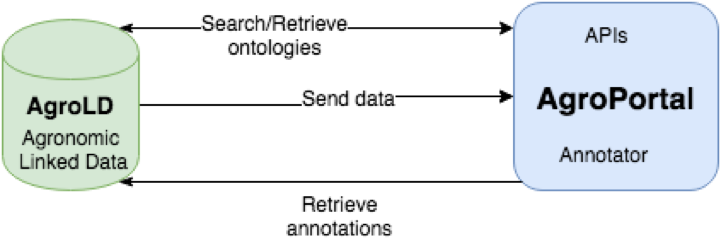
\includegraphics[width=0.70\textwidth]{Figures/AgroPortal-AgroLD.png}
\end{center}
\caption{\label{AgroPortal-AgroLD} Processus d'annotation sémantique entre AgroPortal et AgroLD}
\end{figure}

Le projet AgroLD nous a permis d’identifier de nombreux challenges sur le plan informatique ouvrant de nouvelles pistes de travail. Ces pistes seront plus amplement détaillées dans le projet scientifique. Dans le domaine de la Recherche d’Information nous avons commencé à travailler sur l’indexation des graphes RDF et leur enrichissement sémantique (2016-04). % je mettrai  test de référence (gold standard (en italique et une note pour expliquer)
Nous avons également développé un gold standard pour l’évaluation de méthodes de traduction langage naturel en SPARQL (2016-05). Dans le domaine de l’extraction de connaissances, nous avons évalué l’état de l’art des approches NLP sur les champs littéraux des graphes RDF afin d’enrichir des données liées. Enfin dans le domaine de la reproductibilité des workflows scientifiques, nous avons évalué les différents standards de provenance pouvant être utiliser pour annoter les modèles (2017-02). 
%NLP Natural Language Ptocessing  mais mettre en français traitement automatique de la langue

\subsubsection*{Sélection de références} 
\begin{itemize}

\item (2017-07) Larmande P., El Hassouni N. , Venkatesan A., Tagny G., Ruiz M. The Agronomic Linked Data project (AgroLD) a knowledge network platform for rice. Oral presentation at International Symposium on Rice Functional Genomics ISRFG 2017. Sewon (Korea)
\item (2017-06) Venkatesan A., Tagny G., El Hassouni N., Ruiz M., Larmande P. The Agronomic Linked Data project. Computer demo at Plant and Animal Genomes Conference PAG 2017. San Diego, (USA).
\item  (2017-05) Venkatesan A., Tagny G., El Hassouni N., Chentli I., Guignon V., Ruiz M., Valduriez P. and Larmande P. Agronomic Linked Data: an integrated knowledge system for agronomic research. Plos One (Under review)
\item (2017-04) Dzale Yeumo E, Alaux M, Arnaud E, Aubin S, Baumann U, Buche P, et al. Developing data interoperability using standards: A wheat community use case. F1000Research. 2017;6:1843.
\item (2017-03) Jonquet C, Toulet A, Arnaud E, Aubin E, Dzalé-Yeumo E, Emonet V, Graybeal J, Laporte M-A, Musen M, Pesce V, Larmande P. AgroPortal: an ontology repository for agronomy. Computers and Electronics in Agriculture. 2018. 144:126-143 Impact Factor: 2.201
\item (2017-02) Cohen-Boulakia S, Belhajjame K, Collin O, Chopard J, Froidevaux C, Gaignard A, et al. Scientific workflows for computational reproducibility in the life sciences: Status, challenges and opportunities. Futur. Gener. Comput. Syst. 2017;75. Impact Factor: 2.786
\item (2017-01) Ngompé GT, Venkatesan A, Hassouni N, Ruiz M, Larmande P. AgroLD API Une architecture orientée services pour l’extraction de connaissances dans la base de données liées AgroLD. Lavoisier. 2016. 21:133–58. Impact Factor: 1.046
\item (2016-03) Jonquet C, Toulet A, Arnaud E, Aubin S, Yeumo ED, Emonet V, Graybeal J, Musen MA, Pommier C, Larmande P.  2016.  D202: Reusing the NCBO BioPortal technology for agronomy to build AgroPortal. Oral Presentation at International Conference on Biomedical Ontology and BioCreative ICBO BioCreative 2016. Corvalis (USA)
\item (2016-04) Zevio S., El Hassouni N., Ruiz M. and Larmande P. AgroLD indexing tools with ontological annotations. Poster at Semantic Web for Life Science SWAT4LS 2016. Cambridge (UK)
\item (2016-05) Imène Chentli, Pierre Larmande et Konstantin Todorov. Construction d’un gold standard pour les données agronomiques. IC2016, Montpellier, France.
\item (2016-06) Dagmara Robakowska Hyzorek, Marie Mirouze, Pierre Larmande. Integration and Visualization of Epigenome and Mobilome Data in Crops. Journées ouvertes pour la Biologie, l’informatique et les Mathématiques (JOBIM). Lyon, 2016.
\end{itemize}


\section{Investissements au sein de projets scientifiques}
\begin{itemize}
\item Membre du projet ANR PRCE Data to Knowledge in Agriculture and Biodiversity - D2KAB. 850 K euros. Porteur C. Jonquet. (Soumis en phase 2)
\item Membre du projet international CGIAR – CRP-RICE. 1,5 M euros pour IRD (2017-2022)
\item Membre du projet postdoc Labex Numev. Lingua 75 K euros. Porteur C. Jonquet
\item Porteur du projet Rice-IS – AAP Open Science Labex Agropolis – Search Engine and Analysis Tools for Rice Data. 227 K euros (Rejete)
\item Porteur du projet BIOeSAI Spirale IRD 2014-2015 pour le Développement d’une application de gestion de données phénotypique chez le riz. 11 K euros 
\item Porteur du projet postdoc Labex Numev. LandPan TOGGLE. 2015-2016. 50 K euros (coord. P. Larmande \& F. Sabot).

\item Porteur du projet postdoc Labex Numev. AgroPortal: an ontology repository for agronomy. 2015-2016. 50 K euros (coord. P. Larmande \& C. Jonquet).

\item Membre du projet ANR Investissement d’Avenir IBC « Institut de Biologie Computationnelle » Modélisation, traitement et analyse des données à grande échelle en biologie, santé, agronomie et environnement. 2012-2017. 2.842 M euros. (Coord. WP5 P. Larmande \& P. Valduriez)

\item Membre du projet IFB plant node  (Institut Francais de Bioinformatique).  Développement d’un réseau de ressources bioinformatiques sémantiquement interconnectées. (INRA – CIRAD – CNRS – INRIA  - IRD). 2014-2018. 400 K euros.  (coord. M. Ruiz) 

\item Membre du projet ANR Bioadapt Africrop  « Documenting African Crop Domestication » Partenaires IRD, CIRAD (Coord Y. Vigouroux) 2013-2017. 698 K euros
\item Membre du projet EvoRepRice : « Studying the evolution of reproductive development in the Oryza genus for the improvement of modern cultivated rice ». (coord.  S. Jouannic \& M. Kater) 2010-2014.  479 K euros
\item Membre du projet MENERGEP « Methodologies and new resources for genotyping and phenotyping of African rice species and their pathogens for developing strategic disease resistance breeding programs». Partners: IRD (DIADE), CIRAD (BGPI), Africarice (A. Ghesquière Coord.) projet CGIAR GRISP 800 K\$ US
\end{itemize}

\section{Responsabilité d'animation de la recherche}

\subsection*{Responsabilité d’équipe}
\subsubsection*{Co-Direction ICT Lab USTH - Hanoi} 
Depuis 2017, suite au depart d’Alexis Drogoul à la repésentation IRD Vietnam, j’ai pris la co-direction du laboratoire mixte IRD-USTH ICT Lab\footnote{\url{http://ictlab.usth.edu.vn}} . Il est composé de 11 chercheurs et enseignants chercheurs. Mon rôle comprend en particulier l’animation scientifique, la gestion du budget, les rapports d’activité, la communication. J’y suis également impliqué afin de développer mon projet de recherche notamment en developpant des collaborations avec les membres du laboratoire. 
% J'y suis ...  mal dit..  peut être dire cela implique au delà l'idée de développer le projet de recherche en m'appuyant sur les collaboration au sein du laboratoire.

\subsubsection*{Co-responsable du WP5 de l’Institut de Biologie Computationnelle - IBC} 
Entre mi-2013 et debut 2017, j’ai été coordinateur de l’axe wp5 « intégration des données et connaissances biologiques » d'IBC\footnote{\url{http://www.ibc-montpellier.fr}}. L’objectif de cet axe est de faciliter l’accès aux données et connaissances en biologie. Il est composé de 10 chercheurs et ingénieurs collaborant sur plusieurs projets. Mon rôle de coordination comprenait en particulier le suivi des avancements et des livrables, la gestion du budget, les rapports d’activité, la communication. J’y ai également développé de nouvelles méthodes d’intégration sur des données réelles. De plus, j’ai supervisé le travail d’un post doctorant, d’un ingénieur et de stagiaires afin de travailler sur les différents livrables.  


\subsubsection*{Co-responsable du plateau bioinformatique \textit{i-Trop} IRD} 
Le plateau  \textit{i-Trop}\footnote{\url{http://bioinfo.mpl.ird.fr}} est une infrastructure de calcul et de services mise en place et maintenue par le centre IRD de Montpellier pour les unités locales et les partenaires du sud. Les missions de ce plateau sont (i) de proposer un environnement de travail doté de capacité de calcul et de stockage adapté aux besoins des scientifiques, (ii) de centraliser les ressources bioinformatiques nécessaires pour les utilisateurs du plateau. Depuis janvier 2010, j’ai participé au montage et l’animation de cette structure, dont j’ai été le coordinateur en 2012-2013. Je suis actuellement contributeur en termes de services et applications.


\subsection*{Responsable et Membre de Comités d’Organisation}

\subsubsection*{Semantic Web for Biodiversity (S4BIODIV) 2013 } 
S4BIODIV\footnote{\url{http://semantic-biodiversity.mpl.ird.fr}} est un workshop attaché à la conférence ESWC2013. J'ai Co-organisé le workshop avec E.Arnaud, C. Jonquet, T. Libourel, I. Mougenot, M. Ruiz. Montpellier, France.  Proceedings disponibles sur CEUR\footnote{\url{http://ceur-ws.org/Vol-979/}}

\subsubsection*{PhenoHarmonis : Harmonization, semantic and interoperability of phenotypic and agronomic data Workshop 2014 - 2016 - 2018} Suite au succés du workshop S4BIODIV, le groupe d'organisation a travaillé sur cette nouvelle série.  J'ai co-organisé PhenoHarmonIS\footnote{\url{https://tinyurl.com/PhenoharmonIS2018}} avec E. Arnaud, M. Ruiz, P. Neveu, C. Pommier, D. Pot, JF Rami. Montpellier, France.


\subsubsection*{IC2016 : 27e Journées francophones d'Ingénierie des Connaissances  2016 } 6-10 juin. Montpellier, France.  J'ai pu co-organiser la conference en recherchant des financements permettant d'inviter des keynotes speakers. 
 \footnote{\url{https://ic2016.sciencesconf.org}}

\subsubsection*{AgroHackathon: discovering AgroPortal \& AgroLD. 2016 } Premier Hackathon\footnote{\url{https://www.meetup.com/AgroHackathon}} dédié à l’intégration de données agronomiques. Co-organisation avec C. Jonquet. Montpellier, France.


\subsubsection*{RDA Rice Data Interoperability Working Group} Research Data Alliance est une organisation internationale dont l'objectif est de promouvoir les standards d’échange et la publication des données dans la communauté scientifique. Je coordonne depuis janvier 2017, le groupe pour le riz. l'objectif Rice Data Interoperability WG\footnote{\url{https://www.rd-alliance.org/groups/rice-data-interoperability-wg.html}} sera de proposer l’utilisation de standards et un guide de bonnes pratiques pour échanger et publier les données produites sur le riz. 


% mettre du plus ancien au plus recent
\section{Activités d’enseignement}
\begin{itemize}
\item Enseignement de Bioinformatique au Master 2 ICT USTH, \& Bio, 2017-2018 (50h)
\item Enseignement au Master 2 ICT USTH, Systemes d’information Geographique, 2017 (25h)
\item Enseignement au DESS de Bioinformatique, UMII, TP BioPerl, 2002-2003 (50h)
\item Enseignement IUT Informatique, UMII, TP Base de données, 2004-2006 (120h)
\item Enseignement Master BioPharma USTH (Hanoi), Module Bioinformatique 2013 (40h)
\end{itemize}


\section{Encadrements}

\subsection*{Thèses}

\subsubsection*{2009-2011 J. Wollbrett}
\textit{Title:} Génération semi-automatique de services Web sémantiques pour des bases de données relationnelles biologiques

\begin{itemize}
\item Thèse de l’Université Montpellier II
\item Taux d’encadrement : 50\% avec M.Ruiz et I. Mougenot
\item Soutenance : Dec. 2011
\item Situation actuelle : Post-Doctorant au Swiss Institute of Bioinformatics. Auparavant Post-doctorant au CNRS Roscoff.
\item Financement : Bourse Région LR-CIRAD

\end{itemize}


\subsection*{Stages Post-doctoraux}
% mettre du plus ancien au plus recent

J’ai collaboré avec 3 docteurs en stages post-doctoraux et 2 ingénieurs de recherche.
\begin{description}
\item [+] [2015 – 2017] N. El Hassouni – Contribution dans le développement du projet AgroLD. Financement INRA sur le projet IFB 
\item [+] [2015 - 2017] A. Toulet – Contribution au développement d’un portail d’ontologies pour l’agronomie basé : AgroPortal. Financement Numev puis IBC
o	Co-supervision avec Clément Jonquet
\item [+] [2014 –2016] G. Sempéré – Conception et développement de l’application Gigwa. Financement Cirad.
\item [+] [2014 - 2016] : A. Venkatesan – Intégation de données utilisant les métadonnees et ontologies pour pour agréger les données de plusieurs ressources hétérogenes. Financement IBC
\item [+] [2012-2013] J.Wollbrett - Automatiser l’intégration de bases de données relationnelles distribuées à travers l’enrichissement sémantique de vues RDF avec BioSemantic – Financement Cirad - IBC
\end{description}

\subsection*{Masters }

J’ai encadré 17 masters.
\subsubsection*{Encadrement de stages de master professionnel}
%Annee en gras
\begin{itemize}
\item 2001 C. Tranchant – Développement d’un système d’information sur la traçabilité des échantillons OGM . DESS IAO UMII \\
Situation suivante : Ingénieur Bioinformatique, IRD

\item 2002 G. Droc – Développement d’un pipeline de traitement des séquences génomiques pour les mutants d’insertion chez le riz – Master2 Bioinformatique UMII\\
situation suivante : Ingénieur Bioinformatique, Cirad

\item 2014 F. Philippe -  Analyse de données de variations génétique dans les riz – Master2 bioinformatique Lumini \\
co-encadrement : G. Sempere – Cirad \\
Situation suivante : Ingénieur Bioinformatique, INRA

\item 2017 B. Vautrin – Développement de module ETL pour l’intégration de ressources dans AgroLD. PolyTech. (stage international - Hanoi) \\
Situation suivante : Dernière année polytech 

\item 2017 J-C Idjellidaine – Propososition d’un systeme de recommandation pour valider les mappings sémantiques dans AgroLD. L3 informatique \\
co-encadrement : N. El Hassouni \\
Situation suivante : M1 AIGLE 

\item 2016 A. Petel – Contribution au développement de Gigwa – Master2 Polytech Grenoble \\
co-encadrement : G. Sempéré \\
Situation suivante : Volontaire International Cirad, la Reunion

\item 2016 D. Hyżorek - Epigenetic Data Integration and Analysis – Master2 parcours BCD UM \\
co-encadrement : M. Mirouze \\
Situation suivante : Chercheur en Pologne
\end{itemize}


%annee en gras

\subsubsection*{Encadrement de stages de master recherche}

\begin{itemize}
\item 2007 S. Fromentin - Développement d’un Framework de services web pour l’interopérabilité de ressources agronomiques - Master2 Bioinformatique Orsay\\
Situation suivante : Consultant Bioinformatique SS2I

\item 2008 J. Wollbrett - Intégration automatique d’une ontologie de domaine dans un annuaire de service web bioinformatique : Biomoby – Master2 Bioinformatique UMII\\
co-encadrement : M. Ruiz – Cirad\\
Situation suivante : Thèse CIRAD-Région LR

\item 2014 G. Tagny (M1) - Développement d’une base de connaissance sur les gènes régulateurs de la ramification chez le riz – Master1 Institut Francophone d’Informatique – Hanoi \\
Situation suivante : Master 2

\item 2014 L. Le Ngoc (M1) - Développement d’une application de gestion de données phénotypique chez le riz – Master1 Institut Francophone d’Informatique – Hanoi \\
Situation suivante : Master 2

\item 2015 I. Chentli - Facilitation de l'accès aux données biologiques sémantiquement structurées – Master2 parcours BCD UM \\
co-encadrement : K. Todorov \\
Situation suivante : Ingénieur Bioinformatique, IMGT-CNRS

\item 2015 L. Le Ngoc (M2) - Développement d’un système connaissances pour BIG DATA : application aux données de phénotypage chez le riz (O. sativa) – Master2 Institut Francophone d’Informatique – Hanoi \\
Co-encadrement: 	Pascal Neveu – INRA \\
Situation suivante : Thèse CIFRE Crédit Agricole, Brest

\item 2015 G. Tagny (M2) - The Agronomic Linked Data (AgroLD) project. Master2 Institut Francophone d’Informatique – Hanoi \\
Co-encadrement : A. Venkatesan \\
Situation suivante : Thèse Ecole des Mines Ales, Nîmes

\item 2016 S. Remini - Acquisition automatique de connaissances à partir de textes scientifiques – Master2 parcours BCD UM \\
co-encadrement : K. Todorov \\ 
Situation suivante : Recherche d’emploi

\item  2016 S. Zevio - Indexation de données issues du web sémantique dans le domaine agronomique – Master1 parcours DECOL UM \\
Situation suivante : Master 2 DECOL UM 

\item  2017 A. Diouf –  Proposition et implémentation d’algorithmes de liage de données RDF dans AgroLD – M1 BCD \\
co-encadrement : K. Todorov \\
Situation suivante : M2 BCD

\item  2018 A. Sayadi –  Liage de données complementaires dans le contexte d'AgroLD – M2 AIGLE \\
co-encadrement : K. Todorov \\
Situation suivante : Recherche d'emploi

\item  2018 H. Do –  Evaluating Name-Entity Recognition approaches in plant molecular biology – M1 USTH \\
co-encadrement : K. Tanh \\
Situation suivante : M2 USTH

\item  2018 K.M. Djibril –  Ontology Matching tool using AgroPortal API – M2 USTH \\
Situation suivante : Job
\end{itemize}


\section{Autres implications}
\subsection*{Relectures d’articles}
\begin{itemize}
\item Nucleic Acids Research, 
\item Databases, 
\item BMC Bioinformatics, 
\item Current Plant Biology
\end{itemize}

\subsection*{JURYS}
\begin{itemize}
\item Rapporteur de stages de M2 Bio-Informatique (UM) (régulièrement depuis 2002)
\item Jury Masters BioPharma USTH 2017
\item Jury de concours CNRS (Ingénieur d’Etude)
\end{itemize}

\subsection*{Expertises}
\begin{itemize}
\item Membre extérieur de comité d’évaluation des agents CIRAD
\item Membre de comité d'évaluation des départements Bio et ICT USTH
\end{itemize}


\section{Prototypage}
\begin{itemize}
\item  AgroLD\footnote{\url{http://www.agrold.org}} – Visualisation des données sous forme de graphes RDF, constructeur de requêtes, API de services web.
% 
\item GIGWA\footnote{\url{http://gigwa.southgreen.fr}}  – Développement d’une base de données génomiques, constructeur de requêtes, API de services web. Co-encadrement G. Sempere.
% 
\item BIOeSAI\footnote{\url{http://vmbioesai-dev.ird.fr:8080/Syspherice}} - Développement d’une base de données phénotypique, constructeur de requêtes 
\item BioSemantic\footnote{\url{http://www.southgreen.fr/content/biosemantic-tool}} - Développement d’un constructeur de requêtes SPARQL au-dessus de bases de données relationnelles biologiques. Co-encadrement M. Ruiz
%
\item OryGenesDB\footnote{\url{ http://orygenesdb.cirad.fr}} - Développement d’une base de données génomique pour le riz.
\item Oryza Tag line\footnote{\url{http://oryzatagline.cirad.fr}} - Développement d’une base de données de mutant phénotypiques pour le riz.  
\item Détection de motifs « FST » dans les séquences nucléiques du genome Oryza Sativa (Riz)
\end{itemize}
%